% !Mode:: "TeX:UTF-8" 



\BiSection{2.26}{Figures}

\fancyhead[R]{本题2.26由QC.Z完成}



解:

\scalebox{3}{(a)}

修改的电路图见图1

		\begin{figure}[H] %H为当前位置,!htb为忽略美学标准,htbp为浮动图形
	\begin{minipage}{\linewidth}
		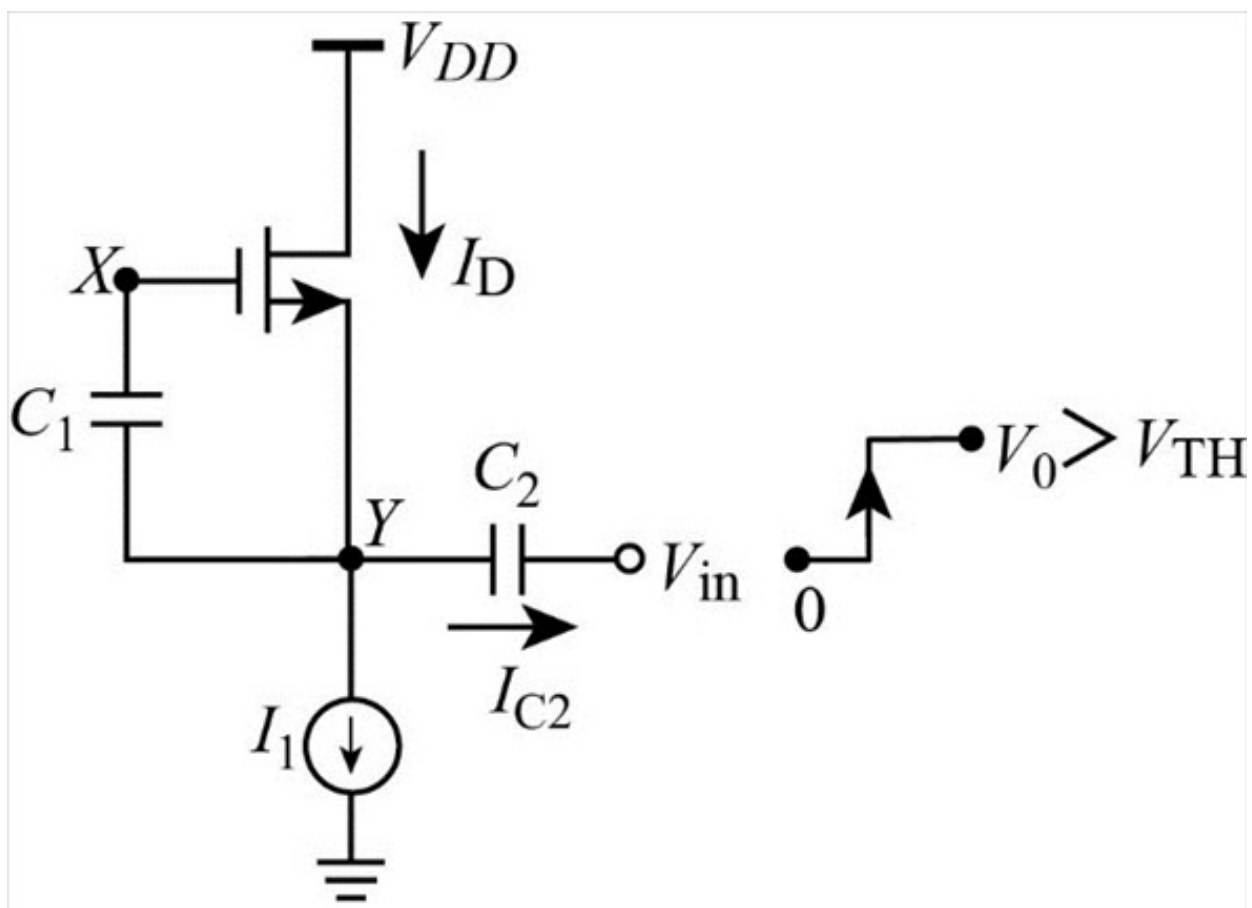
\includegraphics[width=1\linewidth]{2.26-1}
	\end{minipage}
	\caption*{图1} %最终文档中希望显示的图片标题
\end{figure}



\scalebox{2}{(1)}

当$t=0^-$

\begin{figure}[H] %H为当前位置,!htb为忽略美学标准,htbp为浮动图形
	\begin{minipage}{\linewidth}
		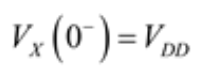
\includegraphics{2.26-2}
	\end{minipage}
\end{figure}

\begin{figure}[H] %H为当前位置,!htb为忽略美学标准,htbp为浮动图形
	\begin{minipage}{\linewidth}
		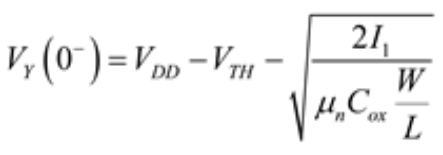
\includegraphics{2.26-3}
	\end{minipage}
\end{figure}

	\color{blue}{
	
	\{
	
	
	$I_1=\frac{1}{2}\mu_nC_{ox}\frac{W}{L}(V_{GS}-V_{TH})^2$
	
	$V_{GS}=V_{TH}+\sqrt{\frac{2I_1}{\mu_nC_{ox}\frac{W}{L}}}$
	
	
	
	
	\}
	
	
	
	
	
	
}









\color{black}{
	
}

\scalebox{2}{(2)}

当$t=0^+$

\begin{figure}[H] %H为当前位置,!htb为忽略美学标准,htbp为浮动图形
	\begin{minipage}{\linewidth}
		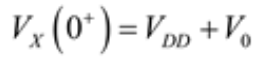
\includegraphics{2.26-4}
	\end{minipage}
\end{figure}

\begin{figure}[H] %H为当前位置,!htb为忽略美学标准,htbp为浮动图形
	\begin{minipage}{\linewidth}
		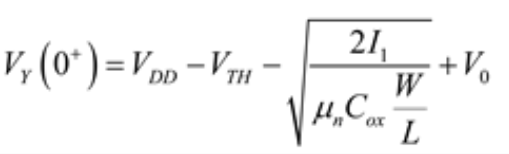
\includegraphics{2.26-5}
	\end{minipage}
\end{figure}

将$V_Y(0^-)$代入上式

\begin{figure}[H] %H为当前位置,!htb为忽略美学标准,htbp为浮动图形
	\begin{minipage}{\linewidth}
		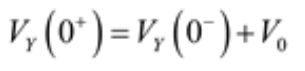
\includegraphics{2.26-6}
	\end{minipage}
\end{figure}

$V_0$是输入电压开始幅度

\scalebox{2}{(3)}

当$t>0$,设$\alpha (t)$是X点电压变化量

\begin{figure}[H] %H为当前位置,!htb为忽略美学标准,htbp为浮动图形
	\begin{minipage}{\linewidth}
		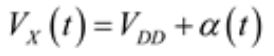
\includegraphics{2.26-7}
	\end{minipage}
\end{figure}

\begin{figure}[H] %H为当前位置,!htb为忽略美学标准,htbp为浮动图形
	\begin{minipage}{\linewidth}
		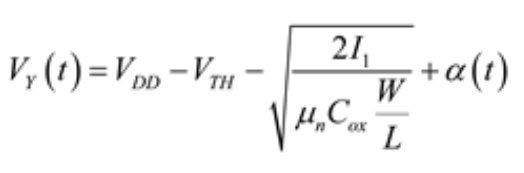
\includegraphics{2.26-8}
	\end{minipage}
\end{figure}

	对图1如果$V_{GS}>V_{TH}+V_{DS}$,NMOS在线性区$I_D=\mu_nC_{ox}\frac{W}{L}[V_{GS}V_{DS}-\frac{1}{2}V_{DS}^2]$
	
	从GS和DS两个方向得Y点电压约束:$V_{DD}-V_{DS}=V_{DD}+\alpha (t)-V_{TH}-\sqrt{\frac{2I_1}{\mu_nC_{ox}\frac{W}{L}}}$
	
	$I_{C2}=C_2\frac{\mathrm{d}\alpha (t)}{\mathrm{d}t}$
	
	$I_{C2}=I_D-I_1$
	
由上四式得$\alpha (t)=V_{TH}+\frac{1}{Kt+\frac{1}{V_0-V_{TH}}}$



\scalebox{2}{(4)}

当$t\rightarrow \infty$

\begin{figure}[H] %H为当前位置,!htb为忽略美学标准,htbp为浮动图形
	\begin{minipage}{\linewidth}
		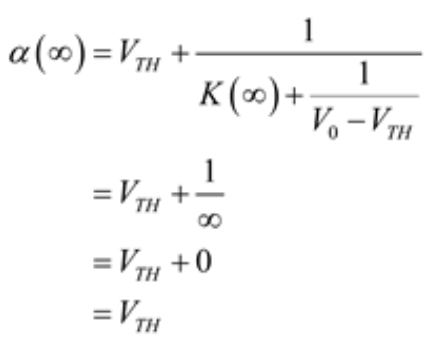
\includegraphics{2.26-9}
	\end{minipage}
\end{figure}

\begin{figure}[H] %H为当前位置,!htb为忽略美学标准,htbp为浮动图形
	\begin{minipage}{\linewidth}
		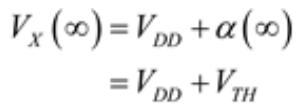
\includegraphics{2.26-10}
	\end{minipage}
\end{figure}

\begin{figure}[H] %H为当前位置,!htb为忽略美学标准,htbp为浮动图形
	\begin{minipage}{\linewidth}
		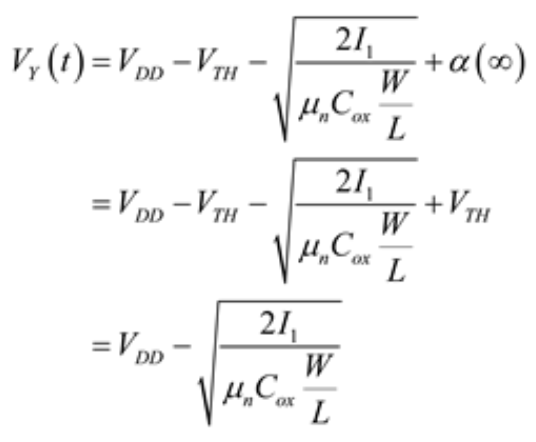
\includegraphics{2.26-11}
	\end{minipage}
\end{figure}

		\begin{figure}[H] %H为当前位置,!htb为忽略美学标准,htbp为浮动图形
	\begin{minipage}{\linewidth}
		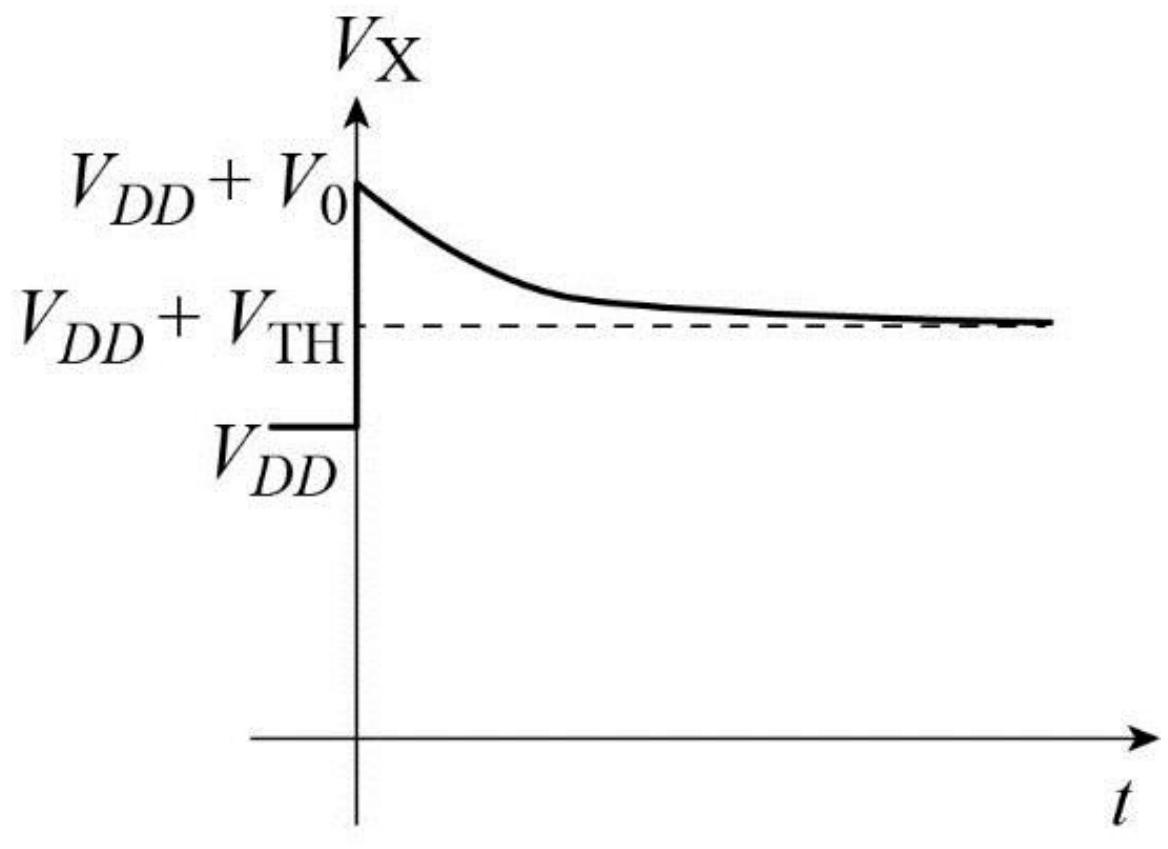
\includegraphics[width=1\linewidth]{2.26-12}
	\end{minipage}
	\caption*{图2} %最终文档中希望显示的图片标题
\end{figure}

		\begin{figure}[H] %H为当前位置,!htb为忽略美学标准,htbp为浮动图形
	\begin{minipage}{\linewidth}
		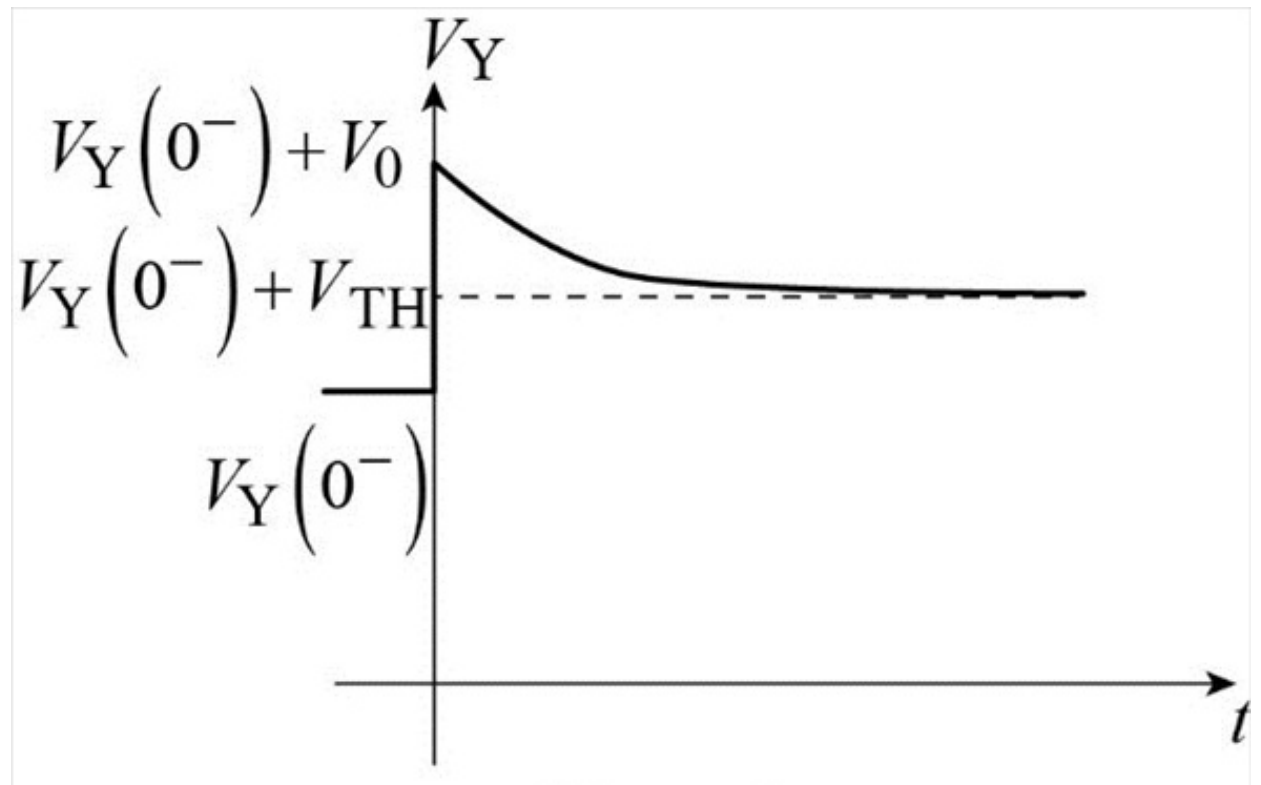
\includegraphics[width=1\linewidth]{2.26-13}
	\end{minipage}
	\caption*{图3} %最终文档中希望显示的图片标题
\end{figure}

	\color{blue}{
	
	\{
	
	
	\scalebox{2}{(3)}
	
	从$V_{DD}-V_{DS}=V_{DD}+\alpha (t)-V_{TH}-\sqrt{\frac{2I_1}{\mu_nC_{ox}\frac{W}{L}}}$解出$V_{DS}$代入$I_D=\mu_nC_{ox}\frac{W}{L}[V_{GS}V_{DS}-\frac{1}{2}V_{DS}^2]$
	
	\begin{figure}[H] %H为当前位置,!htb为忽略美学标准,htbp为浮动图形
		\begin{minipage}{\linewidth}
			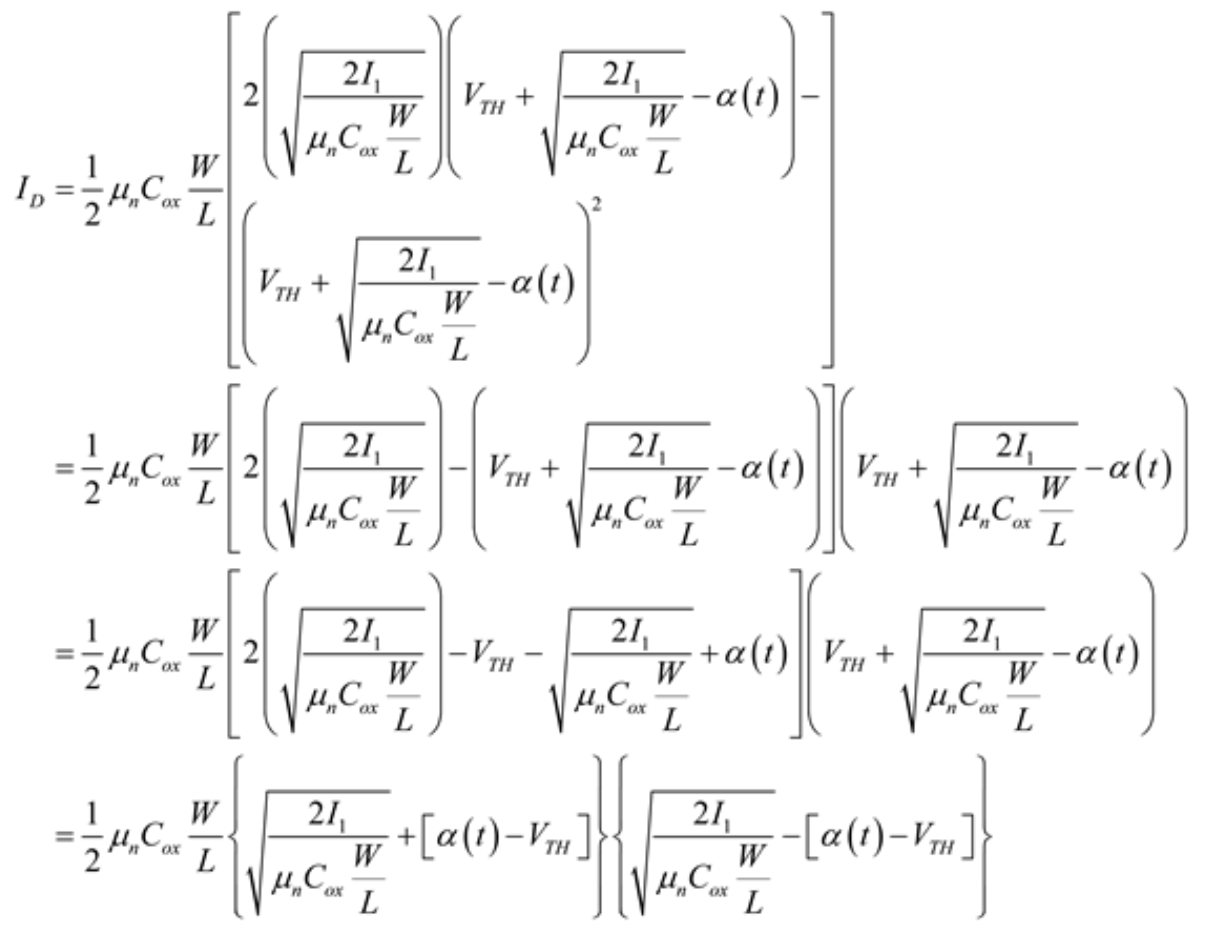
\includegraphics[width=1\linewidth]{2.26-14}
		\end{minipage}
	\end{figure}
	
	\begin{figure}[H] %H为当前位置,!htb为忽略美学标准,htbp为浮动图形
		\begin{minipage}{\linewidth}
			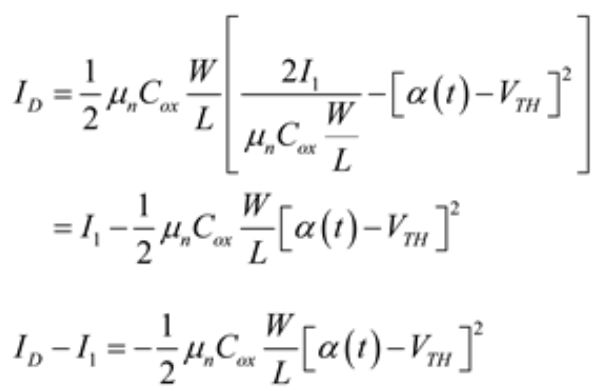
\includegraphics{2.26-15}
		\end{minipage}
	\end{figure}
	
	将$I_{C2}=I_D-I_1$代入上式
	
		\begin{figure}[H] %H为当前位置,!htb为忽略美学标准,htbp为浮动图形
		\begin{minipage}{\linewidth}
			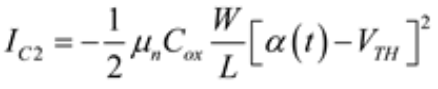
\includegraphics{2.26-16}
		\end{minipage}
	\end{figure}
	
	将$I_{C2}=C_2\frac{\mathrm{d}\alpha (t)}{\mathrm{d}t}$代入上式
	
		\begin{figure}[H] %H为当前位置,!htb为忽略美学标准,htbp为浮动图形
		\begin{minipage}{\linewidth}
			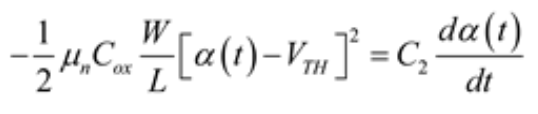
\includegraphics{2.26-17}
		\end{minipage}
	\end{figure}
	
	\begin{figure}[H] %H为当前位置,!htb为忽略美学标准,htbp为浮动图形
		\begin{minipage}{\linewidth}
			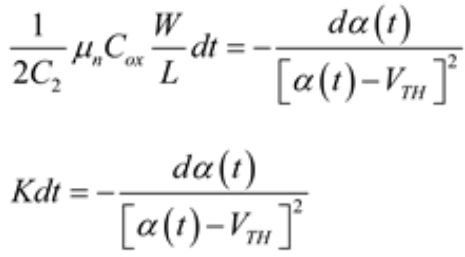
\includegraphics{2.26-18}
		\end{minipage}
	\end{figure}
	
	$k=\frac{1}{2C_2}\mu_nC_{ox}\frac{W}{L}$
	
		\begin{figure}[H] %H为当前位置,!htb为忽略美学标准,htbp为浮动图形
		\begin{minipage}{\linewidth}
			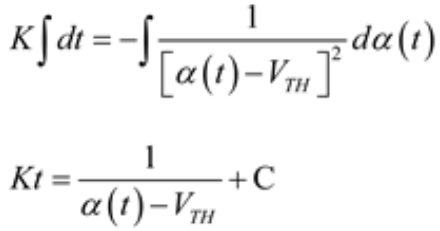
\includegraphics{2.26-19}
		\end{minipage}
	\end{figure}
	
	代入$t=0$解得$C=-\frac{1}{V_0-V_{TH}}$再代回上式
	
			\begin{figure}[H] %H为当前位置,!htb为忽略美学标准,htbp为浮动图形
		\begin{minipage}{\linewidth}
			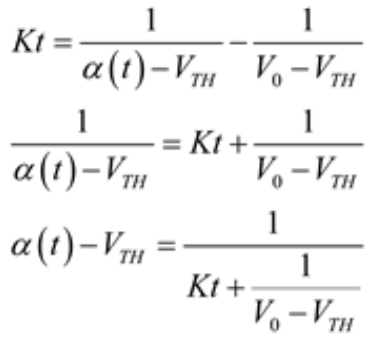
\includegraphics{2.26-20}
		\end{minipage}
	\end{figure}
	
	
	
	
	$\alpha (t)=V_{TH}+\frac{1}{Kt+\frac{1}{V_0-V_{TH}}}$
	
	\}
	
	
	
	
	
	
}









\color{black}{
	
}










\scalebox{3}{(b)}


\scalebox{2}{(1)}

当$t=0^-$

\begin{figure}[H] %H为当前位置,!htb为忽略美学标准,htbp为浮动图形
	\begin{minipage}{\linewidth}
		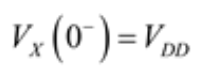
\includegraphics{2.26-2}
	\end{minipage}
\end{figure}

\begin{figure}[H] %H为当前位置,!htb为忽略美学标准,htbp为浮动图形
	\begin{minipage}{\linewidth}
		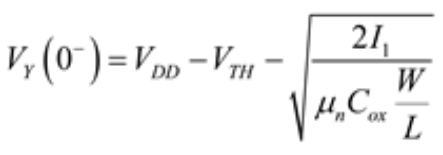
\includegraphics{2.26-3}
	\end{minipage}
\end{figure}

\scalebox{2}{(2)}

当$t=0^+$

\begin{figure}[H] %H为当前位置,!htb为忽略美学标准,htbp为浮动图形
	\begin{minipage}{\linewidth}
		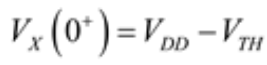
\includegraphics{2.26-21}
	\end{minipage}
\end{figure}

\begin{figure}[H] %H为当前位置,!htb为忽略美学标准,htbp为浮动图形
	\begin{minipage}{\linewidth}
		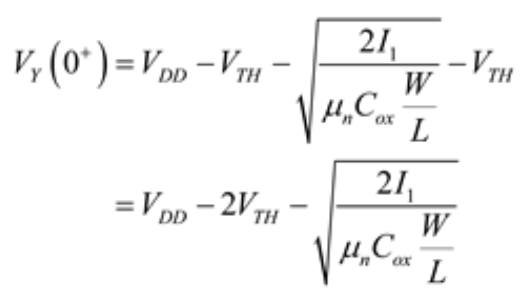
\includegraphics{2.26-22}
	\end{minipage}
\end{figure}

将$V_Y(0^-)$代入上式

\begin{figure}[H] %H为当前位置,!htb为忽略美学标准,htbp为浮动图形
	\begin{minipage}{\linewidth}
		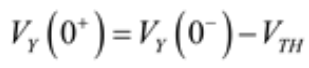
\includegraphics{2.26-23}
	\end{minipage}
\end{figure}

加负阶跃脉冲后NMOS保持在饱和区,电路中的电流不改变,因此$I_{C1}=I_{C2}=0$

		\begin{figure}[H] %H为当前位置,!htb为忽略美学标准,htbp为浮动图形
	\begin{minipage}{\linewidth}
		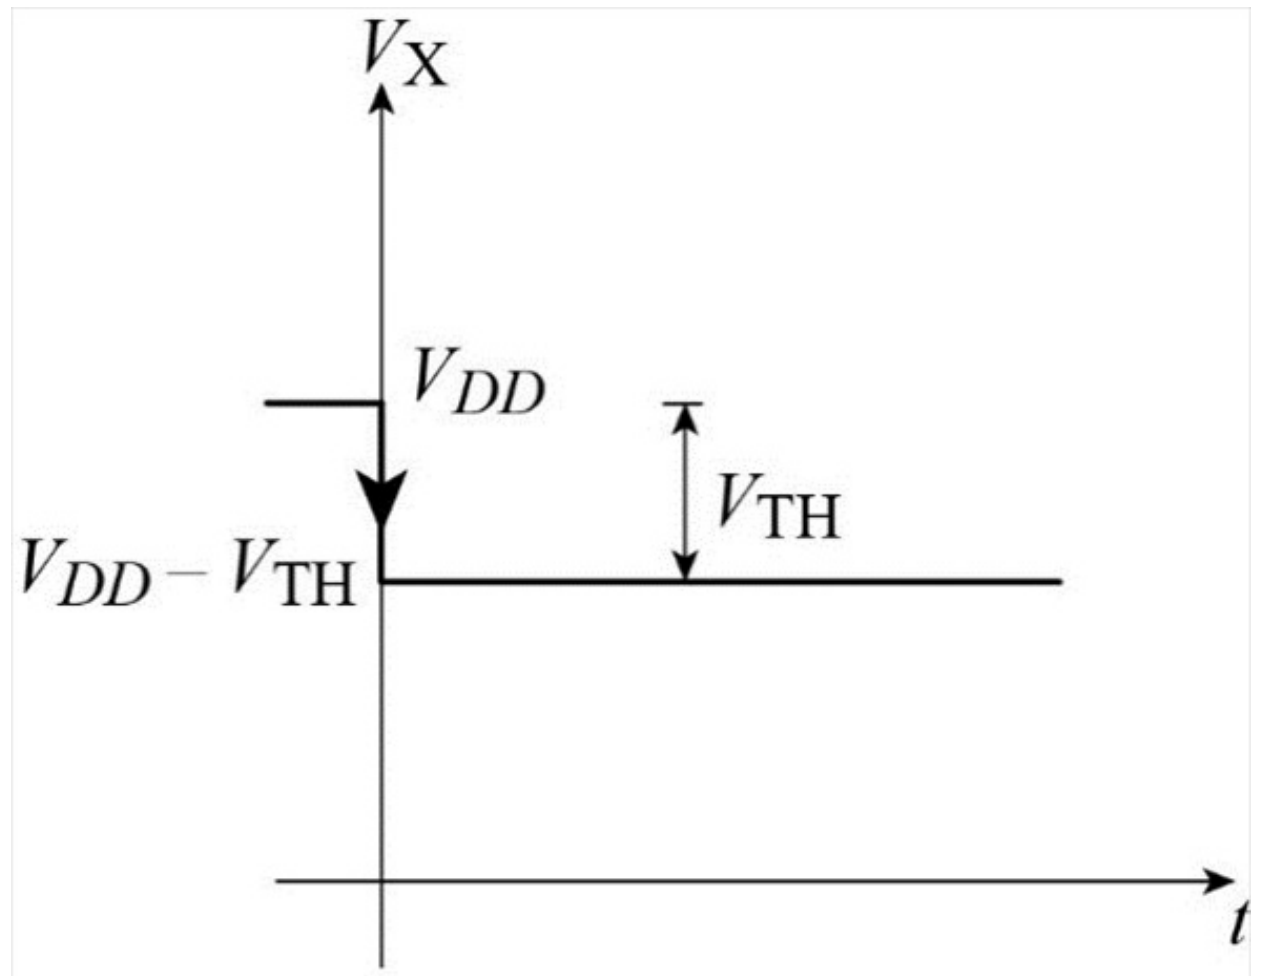
\includegraphics[width=1\linewidth]{2.26-24}
	\end{minipage}
	\caption*{图4} %最终文档中希望显示的图片标题
\end{figure}

\begin{figure}[H] %H为当前位置,!htb为忽略美学标准,htbp为浮动图形
	\begin{minipage}{\linewidth}
		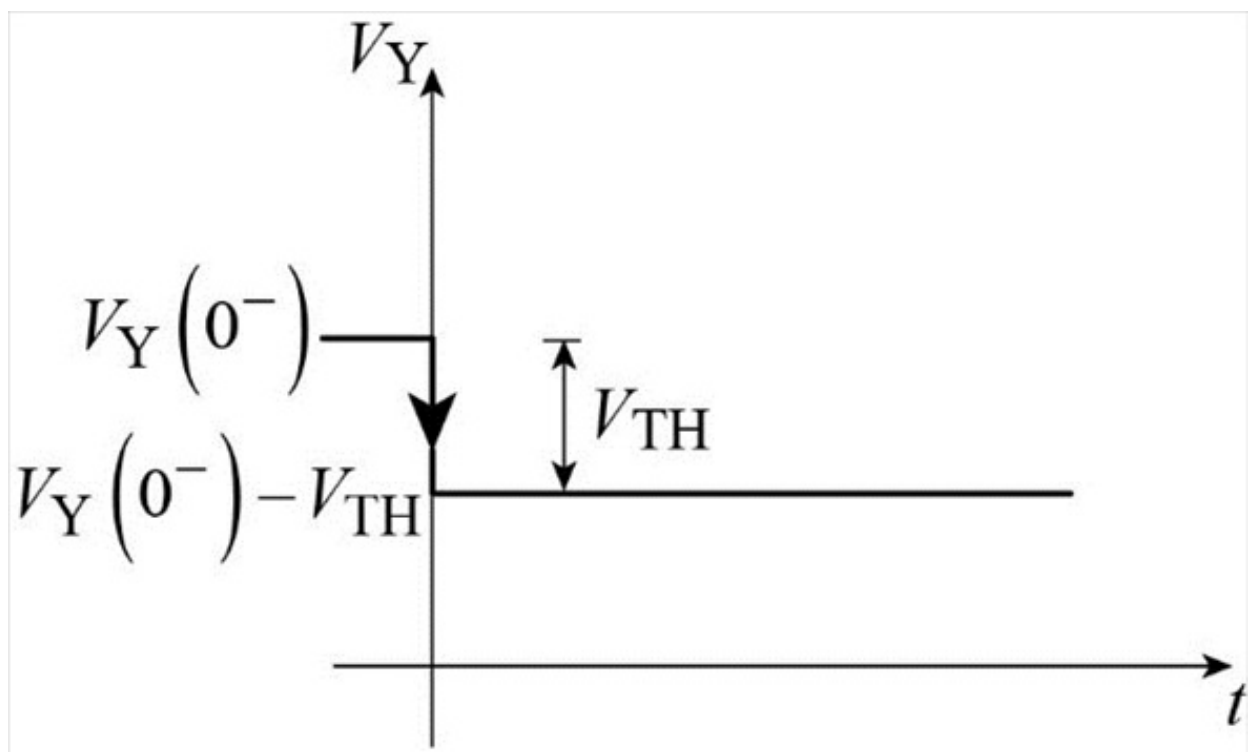
\includegraphics[width=1\linewidth]{2.26-25}
	\end{minipage}
	\caption*{图5} %最终文档中希望显示的图片标题
\end{figure}













	\color{green}{
	
	\{
	
	
	(a)(3)电流线性区但$V_{GS}$饱和区
	
	
	
	
	
	
	\}
	
	
	
	
	
	
}









\color{black}{
	
}